% !TeX root = main.tex

% Requires in the preamble:
% \usepackage{amsmath}
% \usepackage{graphicx}

\section{PER-ACTUATOR FORWARD MODEL: GAUSSIAN PROCESS ARCHITECTURE}
\label{sec:gp_forward_model}

This section defines the forward-model architecture selected for the planar-gait AI controller and states the reasoning behind the choice. The controller follows a latent-space prediction approach: per-actuator forward models are learned in a compact curvature-latent state, composed across actuators, and used to predict and plan the gait. This is a JEPA-inspired, Dreamer-style supervised latent dynamics model~\cite{Assran2025VJEPA2}, not a JEPA in the strict sense, since no representation-learning objective with a stop-gradient EMA target encoder is used.

\subsection{State, Input, and Target Definition}

The gait is produced by five continuous actuators: four legs and one coupled body--tail unit, the latter operated in S-mode only for the planar gait, with channels 5 and 6 alternating and never co-actuated. The suction feet are treated as a scripted binary state and are not modeled dynamically.

The latent state $z$ is the per-actuator constant-curvature parameterization (curvature $\kappa$, or equivalently the bending angle $\theta$ in the actuator body frame), extracted from overhead video of colored actuator stripes after homography rectification to the actuator plane (approximately 8~mm depth). The control input $u$ is the commanded stepper position (equivalently, the displaced syringe volume) per channel; actuation is open-loop, with no pressure sensing and no closed-loop pressure control, so video-derived curvature is the only ground-truth state signal. The forward-model target is the one-step curvature change $\Delta z$, predicted from $(z_t, u_t, \mathrm{dir}_t)$, where $\mathrm{dir}_t$ denotes the direction of the last commanded step and serves as the hysteresis/backlash branch indicator. Training data consists of single-actuator recordings, on the order of tens to hundreds of transitions per actuator; this scale is the primary driver of the architecture decision below.

\subsection{Design Decision: Gaussian Process Forward Model}

Two variants are used and compared empirically. Variant A (prior-based) fits an empirical steps-to-curvature calibration $g_i$ from the actuator's own staircase data (linear, zero-intercept quadratic, or saturating, selected by held-out fit) and places a Gaussian Process (GP) on the residual $\Delta z - \Delta z_{\mathrm{prior}}$. Variant B (model-free) places a GP directly on $\Delta z$ with no prior, against a linear least-squares baseline (B2) and, only if a strong nonlinearity defeats the GP, a small multilayer-perceptron alternative (B3). The winning variant is selected from held-out one-step error, multi-step rollout error, uncertainty calibration, and data-efficiency curves (error versus number of training strokes); the prior-versus-model-free comparison is treated as a result in its own right.

The GP was selected over a neural-network forward model for three reasons tied to the specific data regime of this system. First, the training set is small (tens to hundreds of transitions per actuator); a GP is essentially the data plus a smoothness assumption and has little capacity to overfit at this scale, whereas a multilayer perceptron would require heavy regularization to avoid doing so. Second, a GP posterior provides calibrated predictive uncertainty at no additional cost: variance is small near training data and grows away from it. This property is used directly for planning, since elevated predictive variance during a rollout flags entry into a region the single-actuator data does not cover -- in particular the loaded, closed-chain gait regime, which free-space single-actuator calibration data does not sample. Third, the $O(N^3)$ time and $O(N^2)$ memory cost of exact GP inference, prohibitive at $N \sim 10^6$, is not a constraint at $N$ on the order of a few hundred points.

This choice is not presented as a general claim that GPs are superior to neural forward models. Neural networks dominate at large scale and on high-dimensional, structured inputs (images, text), where a fixed distance-based kernel is not meaningful and learned features are required; those are exactly the regimes in which exact GP inference is infeasible and the curse of dimensionality degrades kernel-based distance. The present setting is the converse: low-dimensional physical state, a few hundred training points, and a task where calibrated uncertainty is directly useful. The prevalence of neural approaches in the wider literature reflects the prevalence of large-scale, high-dimensional problems, not a universal ranking of model classes.

\subsection{Kernel Choice}

The default kernel is Mat\'ern-5/2 with automatic relevance determination (ARD, a separate lengthscale per input dimension), combined with a white-noise term, on standardized inputs. The squared-exponential (RBF) kernel assumes an infinitely smooth latent function,
\begin{equation}
  k_{\mathrm{RBF}}(r) = \sigma_f^2 \exp\!\left(-\frac{r^2}{2\ell^2}\right),
  \label{eqn:gp_rbf_kernel}
\end{equation}
and consequently over-smooths sharp features. The system under study has one such feature: the reversal deadzone associated with mechanical backlash, which produces a near-step change in response at command reversal. The Mat\'ern family is used instead because it does not assume infinite differentiability. The once-differentiable Mat\'ern-3/2 kernel is
\begin{equation}
  k_{3/2}(r) = \sigma_f^2\left(1+\frac{\sqrt{3}r}{\ell}\right)\exp\!\left(-\frac{\sqrt{3}r}{\ell}\right),
  \label{eqn:gp_matern32}
\end{equation}
and the twice-differentiable Mat\'ern-5/2 kernel, used by default, is
\begin{equation}
  k_{5/2}(r) = \sigma_f^2\left(1+\frac{\sqrt{5}r}{\ell}+\frac{5r^2}{3\ell^2}\right)\exp\!\left(-\frac{\sqrt{5}r}{\ell}\right),
  \label{eqn:gp_matern52}
\end{equation}
where $r$ is the distance between input points, $\ell$ is the lengthscale, and $\sigma_f^2$ is the signal variance. The Mat\'ern-3/2 kernel is used on the command axis in place of Mat\'ern-5/2 if the deadzone proves sharper than the twice-differentiable form can represent. As $\nu \to \infty$, the Mat\'ern kernel converges to the RBF kernel in (\ref{eqn:gp_rbf_kernel}). Under ARD, the command dimension is expected to converge to a shorter lengthscale (rougher response) than the smoother state dimensions. The direction feature $\mathrm{dir}_t$ places loading and unloading branches in different regions of input space so that the GP does not average across the deadzone discontinuity. All kernel hyperparameters $(\ell, \sigma_f^2, \sigma_n^2)$ are fit by maximizing the marginal likelihood rather than hand-tuned.

\subsection{Predictive Distribution}

For training inputs $X$ with targets $\mathbf{y} = \Delta z$, a test input $\mathbf{x}_*$, kernel (Gram) matrix $K$, test--train covariance vector $\mathbf{k}_*$, self-covariance $k_{**}$, and noise variance $\sigma_n^2$, the GP posterior predictive mean and variance are~\cite{Rasmussen2006GPML}
\begin{equation}
  \mu(\mathbf{x}_*) = \mathbf{k}_*^{T}\left(K+\sigma_n^2 I\right)^{-1}\mathbf{y},
  \label{eqn:gp_posterior_mean}
\end{equation}
\begin{equation}
  \sigma^2(\mathbf{x}_*) = k_{**} - \mathbf{k}_*^{T}\left(K+\sigma_n^2 I\right)^{-1}\mathbf{k}_*.
  \label{eqn:gp_posterior_variance}
\end{equation}
The mean in (\ref{eqn:gp_posterior_mean}) is a kernel-weighted blend of the training targets; the variance in (\ref{eqn:gp_posterior_variance}) shrinks close to training data and grows away from it, reverting to the prior variance far from any observation.

% --- Figure (schematic, generated from synthetic toy data) ---
\begin{figure}[tb]
  \centering
  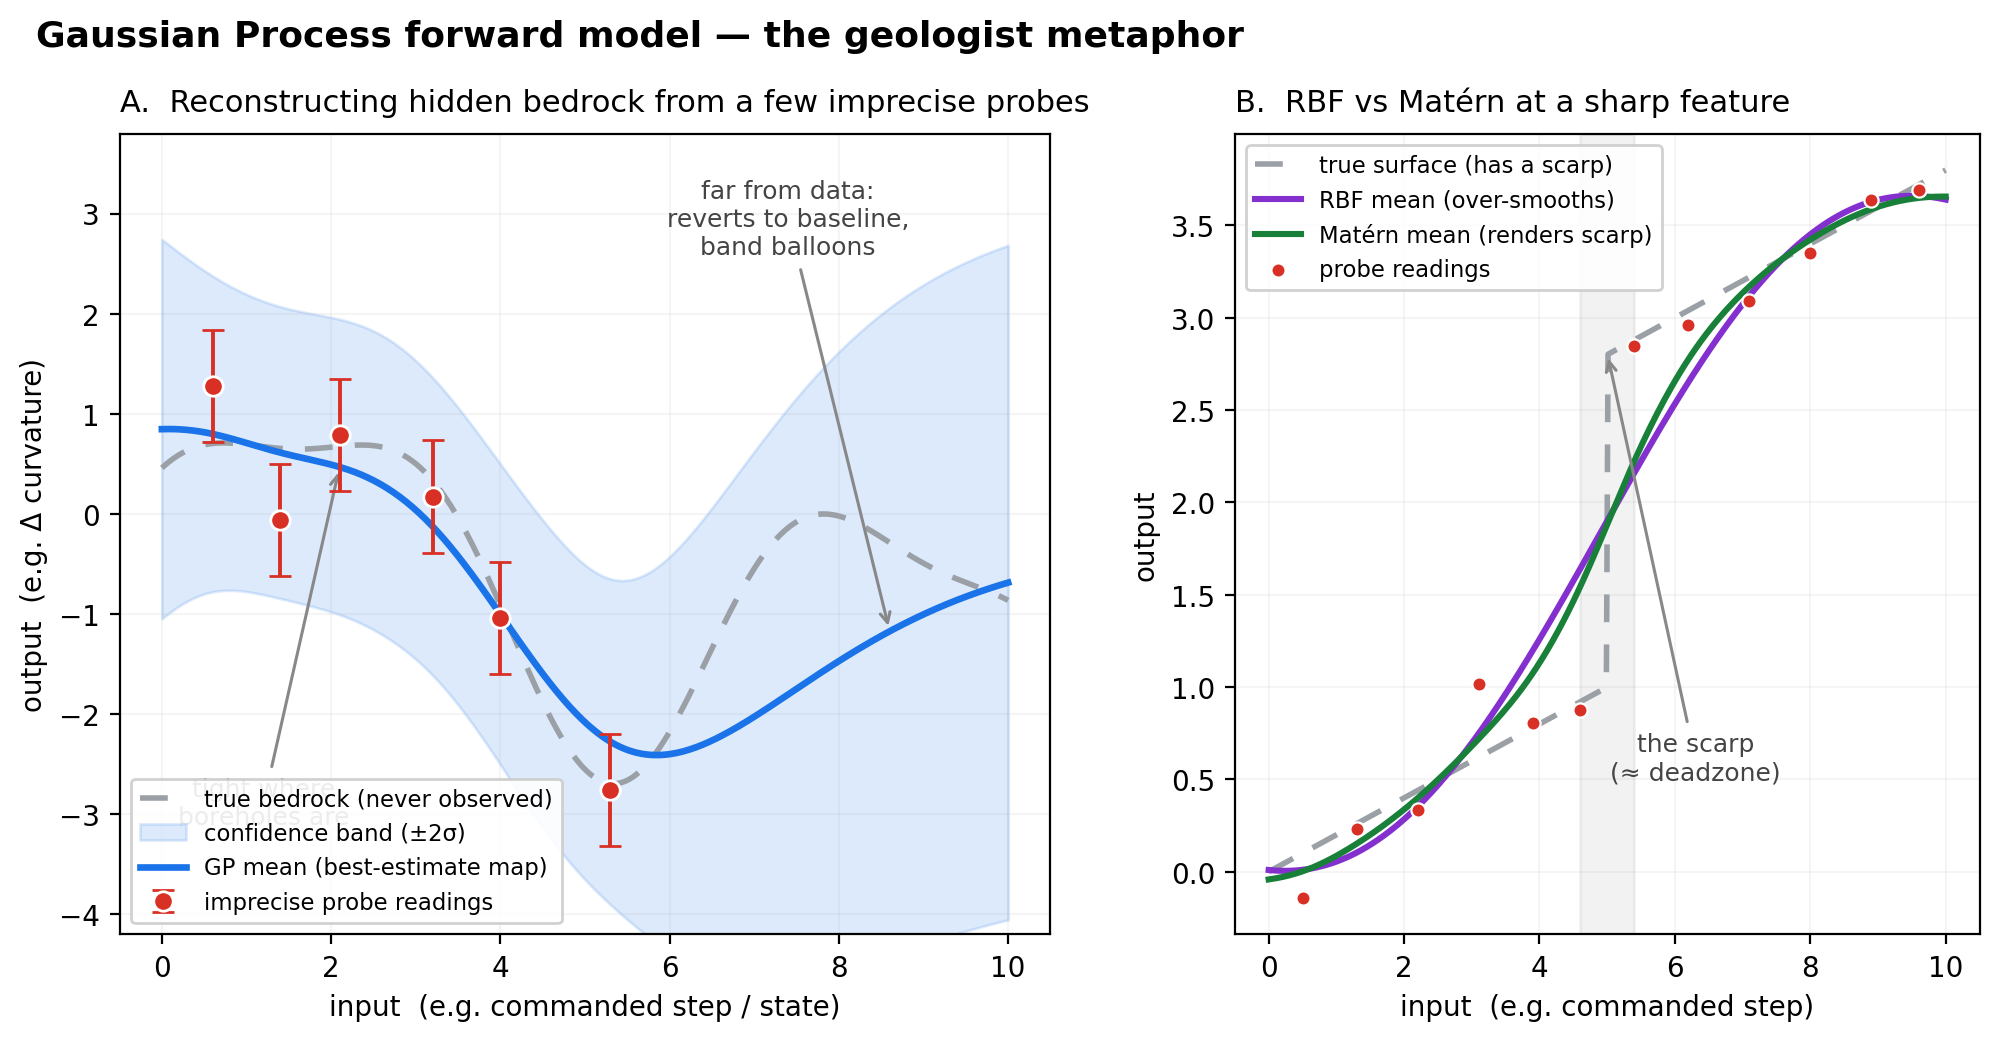
\includegraphics[width=0.9\columnwidth]{figures/gp_geologist_metaphor.png}
  \caption{Schematic illustration of GP mean and uncertainty behavior, generated from synthetic toy data for illustration only. (a) A GP mean fit to a small number of noisy observations, passing near rather than through each point, with the confidence band tight near observations and widening in the data gap, reverting toward the prior mean. (b) RBF versus Mat\'ern-5/2 fit across a step-like feature: the RBF kernel over-smooths the step, while the Mat\'ern-5/2 kernel follows it. \textbf{This figure is a placeholder.} Once single-actuator command--to--curvature-change data is recorded on the robot, an equivalent figure must be regenerated from the real measured transitions, replacing the synthetic bedrock/probe curves with GP fits on real data and the real reversal deadzone.}
  \label{fig:gp_geologist_metaphor}
\end{figure}

\subsection{Related Forward-Model Decisions}

Several subsidiary decisions were fixed alongside the forward-model choice above. The whole-robot forward model composes the five per-actuator predictions plus the scripted suction-foot state structurally, by concatenation; the inter-actuator coupling correction is not itself learned, and the mismatch between the composed model and recorded gait trajectories is instead measured as a transfer residual, treated as a separate planned study. A learned coupling term over gait data is considered only as a stretch goal. The controller built on the composed forward model is likewise not a learned policy network: it is either an open-loop replay of a recorded gait or a sampling-based planner (MPPI or random shooting) over the composed model toward goal keyframes, avoiding a data-hungry learned policy $\pi$.

The reversal deadzone is characterized directly rather than assumed: an ascending/descending command staircase is recorded per actuator, the full stroke transient is logged rather than only the endpoint, and the direction feature $\mathrm{dir}_t$ is included in the model input so that the resulting fit can be validated against the measured loading/unloading gap.

Data augmentation is restricted to truth-injecting transformations: measured-noise input jitter, with the noise level set from the vision pipeline's own centroid/fit-error measurements, and reuse of held-still frames. Autoencoder-noise sampling and hand-interpolation between recorded transitions are excluded, since neither adds dynamical information, and feeding a model's own interpolated outputs back as training data would artificially shrink GP predictive uncertainty and corrupt its calibration. Augmentation is therefore treated as improving precision and robustness only, never coverage; the binding constraint on this forward model is coverage of the loaded, closed-chain gait regime, which only additional near-gait data or a physics-based model can close. Recorded gait trajectories are correspondingly reserved for target definition and evaluation only, and are never used as forward-model training data or augmented.
